Проектируемая система предназначена для выполнения задач управления  робота манипулятором. Нецелесообразно размещать устройства исполнительной управления (ACK) в одном месте ввиду их количества. Поэтому целесообразно решение располагать устройства исполнительной части (ACK) в близи электродвигателя для обеспечения своевременного и точного отклика на управляющие команды, а также для уменьшения электромагнитных помех и потерь мощности на проводах. Так же близкое расположение способствует упрощению обслуживания и повышению надежности системы управления в целом.

\subsection{Gimbal двигатель}

Gimbal электродвигатель в роботе является одним из компонентов механической части оси манипулятора. Двигатель выполняет передачу крутящего момента на ось манипулятора. Это усилие используется для перемещения различных частей робота, таких как звенья и суставы. В большинстве случаев для увеличения крутящего момента между двигателем и осью робота применяется редуктор (или передаточный механизм). Редуктор снижает скорость вращения выходного вала двигателя, увеличивая при этом крутящий момент. Так как прямое соединение двигателя с осью может не обеспечить достаточного усилия или может быть слишком быстрым для точных манипуляций.

Нагрузка, действующая на каждую ось, определяет требуемый крутящий момент, следовательно, был проведен выбор подходящего двигателя и редуктора для каждой оси. Учитывались габариты двигателя, ведь каждое последующее звено, начиная от первой оси и заканчивая последней должно быть легче и компактнее, обусловлено это необходимостью снижения нагрузки на двигатели и распределением массы самой конструкции. Исходя из технических требований, представленных в главе 1, необходимо использовать двигатели нескольких моделей.

Синхронные электродвигатели должны  следующим требованиям :

\begin{itemize}
	\item Внутреннее сопротивление примерно 10 Ом, для уменьшения нагрева электродвигателя с учётом габаритов;
	\item Высокий крутящий момент на низких скоростях, характеристика Kv менее 200 единиц;
	\item Рабочее напряжение от 10 до 20 В;
	\item Малый вес при моменте силы более 1.0 [кгс·см].
\end{itemize}

По результатам анализа моделей с различными параметрами в конструкции робота использовать электродвигатели от карданный шарниров камер (Gimbal). Модели данной категории двигателей обеспечивают оптимальный баланс между крутящим моментом и низкой скоростью вращения. Были выбраны модели GBM4008H-150T, GM5208-120T и GM3506 которые изображены на Рисунке \ref{GBM4008H}. В данных моделях электродвигателей характерной особенностью является количество пар полюсов магнита и катушек ротора - более 20 (Таблица \ref{BLDC}), так как скорость двигателя обратно пропорциональна числу полюсов ротора можно получить больший крутящий момент при низкой скорости вращения двигателя. Данные двигатели имеют большой крутящий момент при сравнительным небольшим весе до 200 граммов. Достоинством данных электродвигателей является широкий диапазон рабочих температур от -20\textdegree  до +60\textdegree \citep{simplefocBLDCMotors}.


\begin{figure}[H]
	\centering
	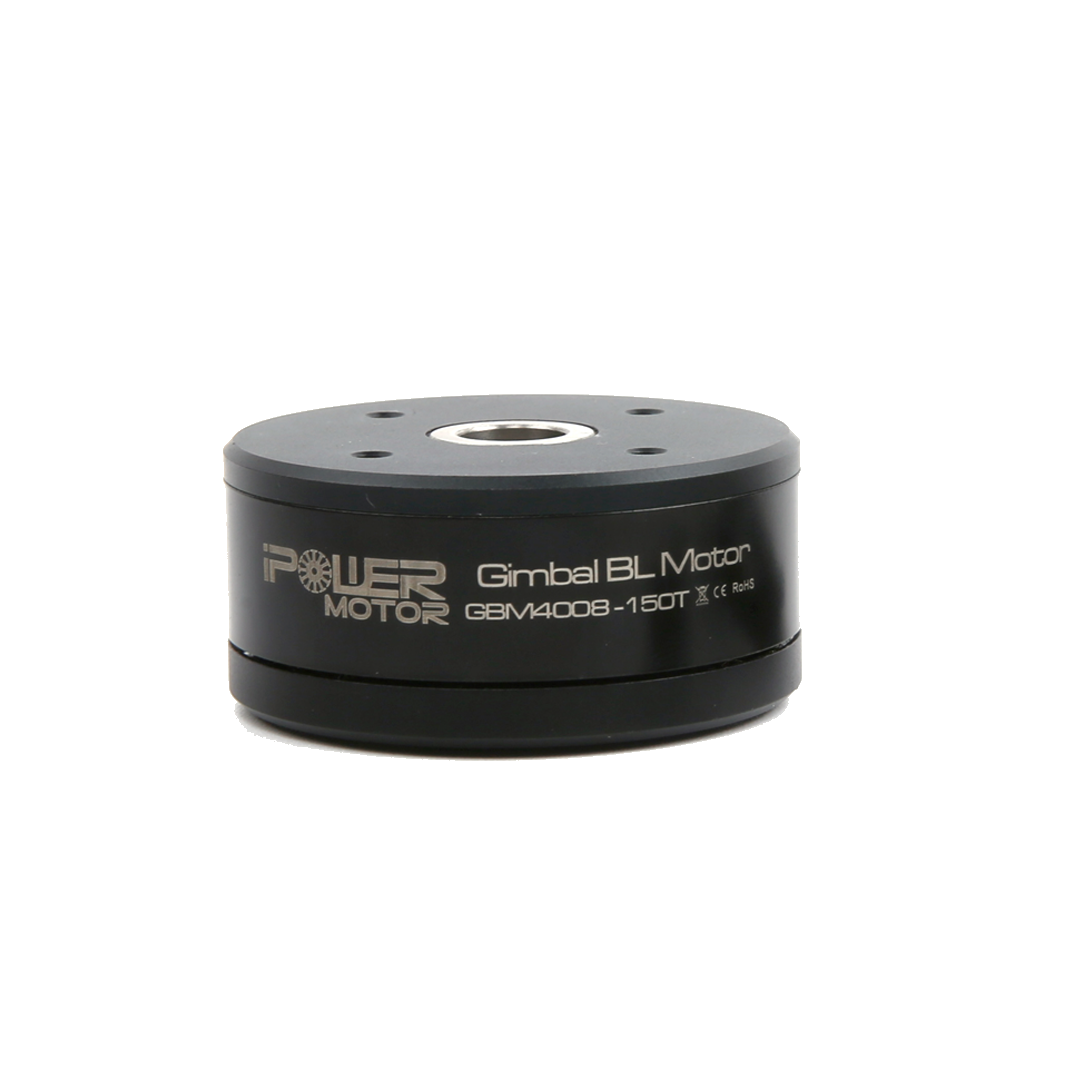
\includegraphics[width=0.5\textwidth]{Src/images/GM4008H-1.png}
	\caption{«BLDC Gimbal motor GBM4008H-150T»}
	\label{GBM4008H}
\end{figure}

 
\begin{table}[H]
	\centering
	\caption{Технические параметры моторов GBM4008H-150T, GM5208-120T и GM3506}\label{BLDC}
	\begin{adjustbox}{width=\textwidth}

		\arrayrulecolor{black}
		\begin{tabular}{!{\color{black}\vrule}l!{\color{black}\vrule}l!{\color{black}\vrule}l!{\color{black}\vrule}l!{\color{black}\vrule}l!{\color{black}\vrule}l!{\color{black}\vrule}l!{\color{black}\vrule}l!{\color{black}\vrule}l!{\color{black}\vrule}}
			\hline
			Model                                                   & \begin{tabular}[c]{@{}l@{}}Diameter~\\{[}mm]\end{tabular} & \begin{tabular}[c]{@{}l@{}}Height~\\{[}mm]\end{tabular} & \begin{tabular}[c]{@{}l@{}}Weight~\\{[}g]\end{tabular} & Kv & \begin{tabular}[c]{@{}l@{}}Poles \&\\Magnets\end{tabular} & \begin{tabular}[c]{@{}l@{}}Resist.~\\{[}ohms]\end{tabular} & \begin{tabular}[c]{@{}l@{}}Torque~\\{[}kgf-cm]\end{tabular} & \begin{tabular}[c]{@{}l@{}}Max				power~\\{[}W]\end{tabular} \\
			\hline
			\begin{tabular}[c]{@{}l@{}}GBM4008H\\-150T\end{tabular} & 46±0.05                                                                         & 21±0.2                                                                        & 107±0.5                                                                      & 68 & 24N22P                                                    & 6.7                                                                              & 1.2                                                                               & 40                                                                                 \\
			\hline
			\begin{tabular}[c]{@{}l@{}}GM5208\\-120T\end{tabular}   & 63±0.05                                                                         & 22.7±0.2                                                                      & 195±0.5                                                                      & 68 & 24N22P                                                    & 6.7                                                                              & 1.9                                                                               & 40                                                                                 \\
			\hline
			GM3506                                                  & 40±0.05                                                                         & 17.8±0.2                                                                      & 64±0.5                                                                       & 40 & 24N22P                                                    & 5.6                                                                              & 1                                                                                 & 25                                                                                 \\
			\hline
		\end{tabular}
	\end{adjustbox}


	\arrayrulecolor{black}
\end{table}


\subsection{Энкодер}

В разработке системы управления робота манипулятора важную роль играет точное определение углов поворота его частей. Так же необходимо определять положение ротора электродвигателя для более плавного управления. Для определения угла поворота обычно используются энкодеры \citep{sciencedirectRobustDesign}.

Одной из важнейшей части является определение позиции каждого звена оси. Критерию точности предъявляется особые требования, исходя из технических требований, необходимо обеспечить точность 0.02 mm на расстоянии 350мм, для обеспечения данной точности необходимо, обеспечить минимальной угол поворота оси на 0.008185°. Разрешение абсолютного энкодера должно соответствовать не менее 16 бит, но энкодеры такого разрешения только начинают появляется и являются дорогим решением в данному применении. Так же стоит учитывать, для векторного регулирования необходимо определять положение ротора двигателя, для обеспечения плавного пуска двигателя. Наилучшим решением двух проблем является установка энкодера на ротор двигателя, а за счет редуктора вырастет не только момент, но и разрешающее способность угла поворота.  Для обеспечения приемлемой точности необходимо использовать редуктор со степенью редукции не менее 11 при разрешении самого энкодера 12 бит. Только необходимо учитывать люфт во всех механических механизмов и устанавливать гармонические или циклоидальные безлюфтовые редукторы \citep{Sensinger2012}


\begin{figure}[H]
	\centering
	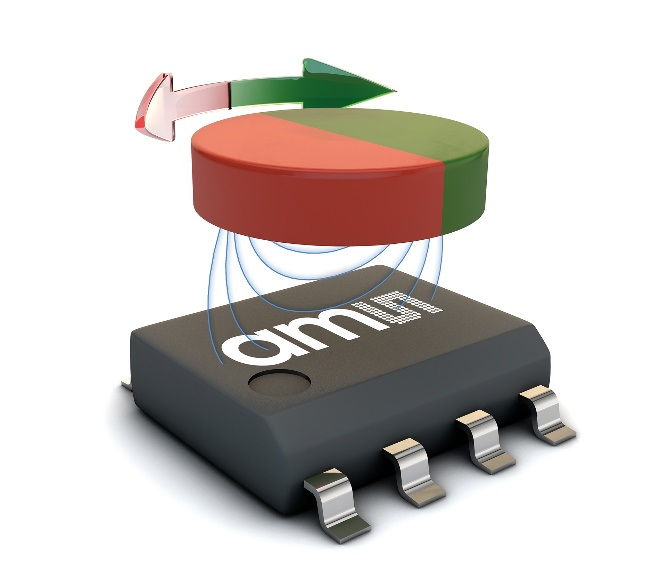
\includegraphics[width=0.5\textwidth]{Src/images/as5600.png}
	\caption{ Микросхема определения осевого положения AS5600}
	\label{as5600P}
\end{figure}

В качестве энкодера была выбрана микросхема AS5600 (Рис. \ref{as5600P}) с цифровым выходом от фирмы «AMS». Датчик магнитного осевого положения AS5600 является бесконтактным датчиком определения абсолютного угла поворота, которая обеспечивает 12 битную точность в измерении углов, в диапазоне от 0 до 360 градусов. AS5600 сочетает в себе надежность и простоту интеграции за счет использования цифрового интерфейса передачи данных I²C (Таблица \ref{as5600T}), что делает его отличным выбором непрерывного и точного контроля за угловым положением оси мотора робота \citep{ams}.

\begin{table}[H]
	\centering
	\caption{Таблица параметров микросхемы осевого положения AS5600}\label{as5600T}
	\begin{tblr}{
		width = \linewidth,
		colspec = {Q[468]Q[445]},
		hlines,
		vlines,
		}
		\textbf{Parameters}       & \textbf{Value} \\
		Resolution				[bit]       & 12             \\
		Output                    & Analog
		out / PWM / I²C                            \\
		Supply				Voltage [V]     & 3-3,6          \\
		Temperature				Range [°C] & -40
		to +125                                    \\
		Package                   & SOIC-8         \\
		Max				current [mA]       & 100            \\
		Sampling				rate [μs]     & 150            \\
		Max
		RPM                       & 20000          \\
		Position				precision [°] & 0.087
	\end{tblr}
\end{table}


\subsection{Устройство стратегического управления}
Устройство стратегического управления необходимо для решения задач движения, а так же является интерфейсом между устройством тактического управления и устройством интеллектуального уровня. Тем самым предоставляя контроль параметрами и управления самим роботом. Устройство стратегического управления должно соответствовать следующим требованиям:
\begin{itemize}
	\item Выполнение нескольких задач одновременно (Многозадачность);
	\item Небольшой размер;
	\item Наличие GPIO;
	\item Высокая вычислительная мощность;
	\item Возможность использования библиотек и функций операционной системы;
	\item Малое напряжение питания;
	\item Поддержание технологий беспроводной связи, спецификации IEEE 802.11 или 802.15.
\end{itemize}

Эти требованием отвечает одноплатный мини-компьютер «Raspberry Pi Zero W 2» (Рисунок \ref{ZeroP}) от компании «Raspberry Pi Foundation». Высокая вычислительная мощность платы (Таблица \ref{ZeroT}) и преимущества операционной системы «Linux» способствуют разработке и выполнению сложных алгоритмов и задач управления на самом устройстве. К тому же поддержка широкого спектра библиотек и доступу к 40-контаткному разъему GPIO из операционной системы, значительно упрощает разработку сложных программ управления и интеграцию с другими системами. В отличии от предыдущих разработок «Raspberry Pi Zero», модификация «Pi Zero 2» имеет более производительный четырехядерный процессор «ARM Cortex-A53» и исправленный дизайн антенны для обеспечения лучшей беспроводной передачи информации.

\begin{figure}[H]
	\centering
	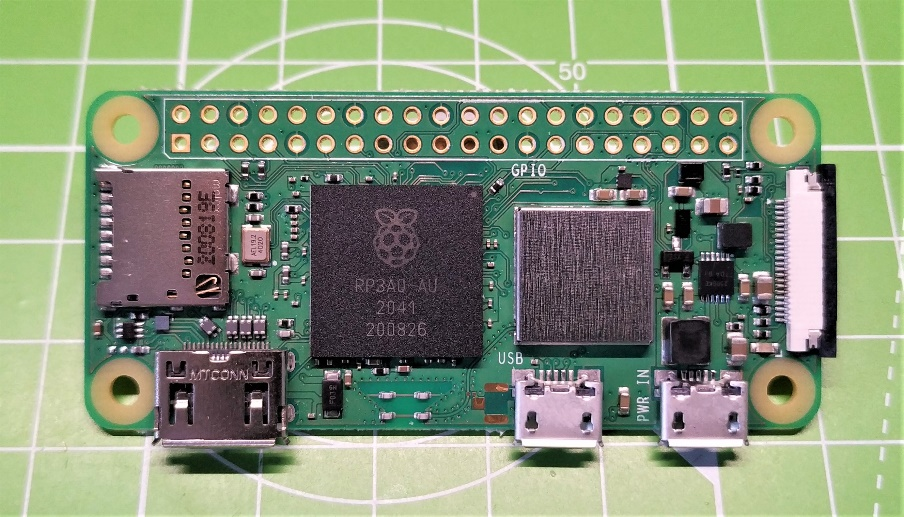
\includegraphics[width=0.6\textwidth]{Src/images/Zero.png}
	\caption{Одноплатного мини-компьютер «Raspberry Pi Zero W 2»}
	\label{ZeroP}
\end{figure}




\begin{table}[H]
	\centering
	\caption{Таблица параметров одноплатного мини-компьютера Raspberry Pi Zero W 2}\label{ZeroT}

	\begin{tblr}{
		width = \linewidth,
		colspec = {Q[180]Q[594]},
		hlines,
		vlines,
		}
		\textbf{Parameters} & \textbf{Value}                      \\
		Processor           & Broadcom
		BCM2710A1, Quad-core Cortex-A53 (ARMv8) 64-bit SoC @ 1GHz \\
		RAM                 & 512MB
		LPDDR2                                                    \\
		Wireless
		Connectivity        & 802.11
		b/g/n wireless LAN, Bluetooth 4.2, BLE                    \\
		Ports               & Mini
		HDMI, USB On-The-Go port, Micro USB power                 \\
		GPIO
		Pins                & 40-pin
		GPIO header                                               \\
		Power
		Requirement         & 5V/2.5A
		DC via micro USB connector or GPIO                        \\
		Size                & 65mm
		x 30mm x 5mm
	\end{tblr}
\end{table}

Основываясь на требованиях к разрабатываемому устройству стратегического управления, с учетом его специфики работы, принято решение использовать операционную систему «Raspberry Pi OS Lite», которая основанная на дистрибутиве «Debian 12» 32-битной версии. Основной особенностью данного дистрибутива является стабильность, безопасность и широкая поддержка пакетов.

\subsection{Контроллер тактического и исполнительного управления}

Согласно требованиях к разрабатываемой системе управления, устройством управления для тактического и исполнительного устройство должно иметь малые габариты поэтому для реализации необходимо использовать микроконтроллер, за счет малых его размера. В задачу микроконтроллера входит: считывание и обработка данных от датчиков, осуществление обмена данными по шине данных, производство численных вычислений для векторного регулирования, прямой и обратной задачи кинематики, а также осуществление генерации сигналов PWM для инвертора. Минимальные требования к микроконтроллеру:
\begin{itemize}
	\item Рабочее питание от 3В;
	\item Наличие более 20 линии ввода/вывода;
	\item Порты для работы с CAN-шиной;
	\item Порты для работы с PWM;
	\item Аппаратная поддержка I2C протокола на выводах МК;
	\item Наличие внутреннего АЦП;
	\item Наличие механизма прямого доступ к памяти DMA.
\end{itemize}

Основной проблемой при выборе микроконтроллера, был недостаток информации применительно к решению задач системы управления тактического и исполнительного управления. Проблема заключалась в выборе лучшей модели МК при решениях кинематических задач. Невозможно было определить какой МК, среди самых распространённых на рынке, имеет лидирующее место. Микроконтроллеры сильно отличаются внутри одного семейства, а при рассмотрении моделей от разных производителей, архитектура каждого МК сильно отличается, надо было учесть и (toolchain) набор инструментов программирования, который тоже мог влиять на производительность. Следовательно, возникла необходимость провести тестирование различных видов микроконтроллеров общего применения, доступных на рынке.

\subsection{Тестирование микроконтроллеров}

Проведённое тестирование было необходимо для нахождения подходящей модели микроконтроллера. Основным критерием выбора была скорость выполнения математических операций. Высокая скорость выполнения необходима для обеспечения эффективной работы системы в реальном времени. Это особенно важно в задаче векторного регулирования, где задержки в обработке данных приводят к существенным потерям точности, а также отзывчивости всей системы в целом.	При более подробном рассмотрение задач связанных с вычислением задач кинематики и векторного регулирования, было обнаружено большое количество вычислений\citep{5899203}:
\begin{itemize}
	\item Умножение и деление чисел с плавающей запятой;
	\item Вычисление тригонометрических выражений, функции синуса и косинуса;
	\item Вычисление квадратного корня.
\end{itemize}

Приведённые выше пункты являются сложными для вычислений на ядре микроконтроллера и нуждаются в большом количестве операций процессора для их вычисления.  Вычисление подобных выражений будет занимать весомое количество времени, чем негативно скажется на быстродействии работы всего управления, так и на работе отдельных её частей\citep{pack2008microcontroller}.


Для проведения теста были выбраны микроконтроллеры от производителей: «STMicro electronics», «Raspberry PI Foundation», «Espressif Systems».
Главным критерием сравнения было измерение затраченного времени на каждый тип вычисления. Во время тестирования не использовались действия, связанные с приостановкой главного цикла исполняемой программы, например прерывания.

\begin{figure}[H]
	\centering
	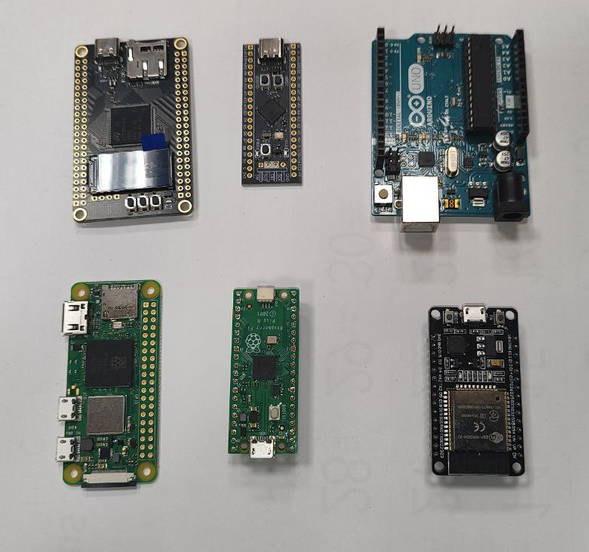
\includegraphics[width=0.4\textwidth]{Src/images/TestDevices.png}
	\caption{Платы, который участвовали в тестировании}
	\label{Test}
\end{figure}

В таблице \ref{TestT} приведен перечень использовавшихся микроконтроллеров, их тактовая частота и процессор. Платы которые участвовали в испытании изображены на рисунке \ref{Test}.

% \usepackage{color}
% \usepackage{tabularray}
\definecolor{DustyGray}{rgb}{0.6,0.6,0.6}
\begin{table}[H]
	\centering
	\caption{Список Микроконтроллеров их характеристки}\label{TestT}
	\begin{tblr}{
		width = \linewidth,
		colspec = {Q[269]Q[274]Q[146]Q[248]},
		hlines,
		vlines = {Black},
		vline{1} = {-}{DustyGray},
		}
		\textbf{Board} & \textbf{MCU}            & \textbf{Fcpu (Mhz)} & \textbf{CPU}                   \\
		Arduino
		Uno (original) & ATmega328p              & 16                  & AVR                            \\
		NodeMCU-ESP32  & ESP32                   & 240                 & Dual
		Xtensa LX6                                                                                      \\
		NodeMcu
		V3             & ESP8266                 & 160                 & Xtensa
		L106                                                                                            \\
		Raspberry
		Pi Pico        & RP2040				[Arduino IDE] & 133                 & Dual
		Cortex M0+                                                                                      \\
		Raspberry
		Pi Pico        & RP2040				[C++ SDK]     & 133                 & Dual
		Cortex M0+                                                                                      \\
		Raspberry
		Pi Pico        & RP2040				[MicroPython] & 133                 & Dual
		Cortex M0+                                                                                      \\
		STM32
		Nucleo-32      & STM32G431KB             & 170                 & Cortex
		M4                                                                                              \\
		STM32
		Nucleo-32      & STM32G431				[FPU-OFF]  & 133                 & Cortex				M4, \textbf{FPU-OFF}
	\end{tblr}
\end{table}

Суть программы в микроконтроллере состояла в вычислении затрачиваемого времени с использованием порта GPIO. Перед вычислением операции выключаются все прерывания, микроконтроллер поднимает сигнал на выводе в высокое состояние, производится вычисление математической операции, на выводе ножки МК опускает в нижнее состояние, прерывания восстанавливаются. Далее при помощи осциллографа HMO2024 от производителя «ROHDE \& SCHWARZ», измерялась длительность импульса и данные записывались в таблицу \ref{TestTimeT}, стоит отметить, что при расчётах учитывалось время переключения выходов GPIO, записанные во 2 колоне таблицы \ref{TestTimeT}, результаты показаны на графике \ref{TestTimeP}.



% \usepackage{color}
% \usepackage{tabularray}

\input{Src/chapters/Colors.tex}

\begin{table}[H]
	\centering
	\caption{Таблица измеренного времени на вычисление математических операций}\label{TestTimeT}

	\begin{adjustbox}{width=\textwidth}

		\begin{tblr}{
				cell{2}{2} = {DeYork},
				cell{2}{3} = {Salomie},
				cell{2}{4} = {Salomie},
				cell{2}{5} = {Salomie1},
				cell{2}{6} = {Salomie2},
				cell{2}{7} = {MacaroniandCheese},
				cell{2}{8} = {MacaroniandCheese1},
				cell{2}{9} = {Salomie2},
				cell{2}{10} = {Carnation},
				cell{3}{2} = {DeYork1},
				cell{3}{3} = {DeYork2},
				cell{3}{4} = {DeYork3},
				cell{3}{5} = {DeYork2},
				cell{3}{6} = {DeYork4},
				cell{3}{7} = {Feijoa},
				cell{3}{8} = {YellowGreen},
				cell{3}{9} = {DeYork5},
				cell{3}{10} = {Salomie3},
				cell{4}{2} = {DeYork6},
				cell{4}{3} = {Feijoa1},
				cell{4}{4} = {Feijoa2},
				cell{4}{5} = {YellowGreen1},
				cell{4}{6} = {Salomie3},
				cell{4}{7} = {Salomie4},
				cell{4}{8} = {Salomie5},
				cell{4}{9} = {Salomie},
				cell{4}{10} = {Chardonnay},
				cell{5}{2} = {DeYork7},
				cell{5}{3} = {YellowGreen2},
				cell{5}{4} = {YellowGreen3},
				cell{5}{5} = {SaharaSand},
				cell{5}{6} = {Salomie3},
				cell{5}{7} = {Salomie6},
				cell{5}{8} = {Salomie7},
				cell{5}{9} = {Salomie3},
				cell{5}{10} = {Grandis},
				cell{6}{2} = {Fern},
				cell{6}{3} = {Feijoa3},
				cell{6}{4} = {Feijoa4},
				cell{6}{5} = {DeYork8},
				cell{6}{6} = {Feijoa5},
				cell{6}{7} = {Salomie8},
				cell{6}{8} = {Salomie8},
				cell{6}{9} = {Feijoa6},
				cell{6}{10} = {Salomie9},
				cell{7}{2} = {Salomie8},
				cell{7}{3} = {Salomie9},
				cell{7}{4} = {Salomie6},
				cell{7}{5} = {Salomie6},
				cell{7}{6} = {Salomie9},
				cell{7}{7} = {Salomie10},
				cell{7}{8} = {Salomie5},
				cell{7}{9} = {Salomie11},
				cell{7}{10} = {Salomie12},
				cell{8}{2} = {Fern},
				cell{8}{3} = {Fern1},
				cell{8}{4} = {Fern1},
				cell{8}{5} = {Fern2},
				cell{8}{6} = {DeYork},
				cell{8}{7} = {DeYork9},
				cell{8}{8} = {Feijoa2},
				cell{8}{9} = {DeYork10},
				cell{8}{10} = {Salomie8},
				cell{9}{2} = {Fern},
				cell{9}{3} = {DeYork6},
				cell{9}{4} = {DeYork11},
				cell{9}{5} = {DeYork12},
				cell{9}{6} = {YellowGreen1},
				cell{9}{7} = {Salomie8},
				cell{9}{8} = {Salomie4},
				cell{9}{9} = {Salomie3},
				cell{9}{10} = {Salomie13},
				hlines,
				vlines,
			}
			MCU                                 & {Time IO\\{[}μs]} & {~a~
			+~ b                                                                                                                                                                                                                                                         \\~[μs]} & {a~ -~ b \\{[}μs]} & {a~
			*~ b\\{[}μs]} & {a~
			/ b\\{[}μs]}  & {sin(a)\\{[}μs]}  & {log(a)\\{[}μs]} & {sqrt(b)\\{[}μs]} & {pow(b, a)\\{[}μs]}                                                 \\
			ATmega328p~                         & 0,144                                   & 9,134                                  & 8,818                                   & 10,141                                    & 31,154 & 104,655 & 155,218 & 31,133 & 328,810 \\
			ESP32                               & 0,312                                   & 0,402                                  & 0,389                                   & 0,399                                     & 0,567  & 0,798   & 1,357   & 0,691  & 3,120   \\
			ESP8266~                            & 0,508                                   & 0,942                                  & 0,959                                   & 1,214                                     & 2,296  & 13,393  & 26,611  & 8,454  & 76,808  \\
			{RP2040~[Arduino IDE]}              & 0,514                                   & 1,477                                  & 1,555                                   & 1,884                                     & 4,233  & 17,052  & 28,012  & 4,090  & 62,245  \\
			{RP2040{[}C++ SDK]}                 & 0,008                                   & 0,750                                  & 0,783                                   & 0,650                                     & 0,819  & 4,634   & 6,610   & 0,709  & 17,288  \\
			{RP2040~[MicroPython]}              & 6,456                                   & 18,412                                 & 17,086                                  & 16,858                                    & 17,499 & 23,491  & 25,253  & 19,688 & 41,450  \\
			STM32G431~                          & 0,005                                   & 0,063                                  & 0,065                                   & 0,056                                     & 0,140  & 0,449   & 0,957   & 0,136  & 5,266   \\
			STM32G431 [FPU-OFF]                 & 0,007                                   & 0,508                                  & 0,529                                   & 0,350                                     & 1,217  & 5,414   & 12,395  & 2,566  & 42,773
		\end{tblr}
	\end{adjustbox}


\end{table}

\definecolor{Fern}{rgb}{0.388,0.745,0.482}

\begin{figure}[H]
	\centering

	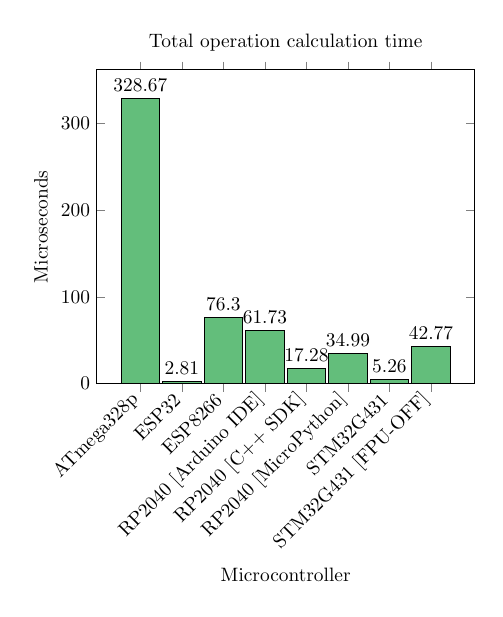
\begin{tikzpicture}[scale=0.7]
		\begin{axis}[
			x tick label style={rotate=45, anchor=east, align=right},
			title=Total operation calculation time,
			xlabel={Microcontroller},
			ylabel={Microseconds},
			ymin=0,
			ybar=5pt, % Adjust the space between bars
			enlarge x limits=0.15, % Add some breathing room between the bars
			bar width=20pt, % Adjust the width of the bars
			symbolic x coords={ATmega328p,ESP32,ESP8266,RP2040 [Arduino IDE],RP2040 [C++ SDK],RP2040 [MicroPython],STM32G431,STM32G431 [FPU-OFF]},
			xtick=data,
			nodes near coords,
			nodes near coords align={vertical},
			]
			\addplot[fill=Fern] coordinates  {
					(ATmega328p,328.667)
					(ESP32,2.808)
					(ESP8266,76.300)
					(RP2040 [Arduino IDE],61.730)
					(RP2040 [C++ SDK],17.280)
					(RP2040 [MicroPython],34.994)
					(STM32G431,5.261)
					(STM32G431 [FPU-OFF],42.766)
				};
		\end{axis}
	\end{tikzpicture}
	\caption{График сравнения времени вычисления математических операций у различных МК}\label{TestTimeP}

\end{figure}


Приведённые данные не дали чёткую информации о преимуществах конкретного контроллера в конкретных вычислениях, для давнейшего и более удобного анализа таблица пересчитана в значения тысяч операций в секунду kOPS, формула(\ref{kops}).

\begin{ceqn}
	\begin{align} \label{kops}
		kOPS= \frac{1000}{T_{cal} - T_{io}}
	\end{align}
\end{ceqn}

% \usepackage{color}
% \usepackage{tabularray}

\begin{table}[H]
	\centering
	\caption{Таблица сравнения тысяч операций в секунду на вычисление математических операций у каждого МК}\label{TestTimeT2}

	\begin{adjustbox}{width=\textwidth}

		\begin{tblr}{
				cell{2}{2} = {Salmon,r},
				cell{2}{3} = {AtomicTangerine,r},
				cell{2}{4} = {Salmon1,r},
				cell{2}{5} = {Froly,r},
				cell{2}{6} = {Carnation,r},
				cell{2}{7} = {Carnation1,r},
				cell{2}{8} = {Froly,r},
				cell{2}{9} = {Carnation2,r},
				cell{3}{2} = {Feijoa,r},
				cell{3}{3} = {Feijoa1,r},
				cell{3}{4} = {Feijoa2,r},
				cell{3}{5} = {Putty,r},
				cell{3}{6} = {SaharaSand,r},
				cell{3}{7} = {SweetCorn,r},
				cell{3}{8} = {Flax,r},
				cell{3}{9} = {Salomie,r},
				cell{4}{2} = {SaharaSand1,r},
				cell{4}{3} = {SaharaSand2,r},
				cell{4}{4} = {SweetCorn1,r},
				cell{4}{5} = {SweetCorn2,r},
				cell{4}{6} = {Salmon2,r},
				cell{4}{7} = {Froly1,r},
				cell{4}{8} = {AtomicTangerine1,r},
				cell{4}{9} = {Carnation3,r},
				cell{5}{2} = {SweetCorn,r},
				cell{5}{3} = {SweetCorn,r},
				cell{5}{4} = {SweetCorn3,r},
				cell{5}{5} = {Salomie1,r},
				cell{5}{6} = {Salmon3,r},
				cell{5}{7} = {Froly2,r},
				cell{5}{8} = {Salomie2,r},
				cell{5}{9} = {Carnation4,r},
				cell{6}{2} = {SweetCorn1,r},
				cell{6}{3} = {SweetCorn4,r},
				cell{6}{4} = {SaharaSand3,r},
				cell{6}{5} = {SweetCorn4,r},
				cell{6}{6} = {MacaroniandCheese,r},
				cell{6}{7} = {HitPink,r},
				cell{6}{8} = {SweetCorn5,r},
				cell{6}{9} = {Froly3,r},
				cell{7}{2} = {Salmon4,r},
				cell{7}{3} = {Salmon5,r},
				cell{7}{4} = {Salmon6,r},
				cell{7}{5} = {Salmon7,r},
				cell{7}{6} = {Froly3,r},
				cell{7}{7} = {Froly4,r},
				cell{7}{8} = {Salmon8,r},
				cell{7}{9} = {Froly5,r},
				cell{8}{2} = {DeYork,r},
				cell{8}{3} = {DeYork1,r},
				cell{8}{4} = {Fern,r},
				cell{8}{5} = {YellowGreen,r},
				cell{8}{6} = {SaharaSand2,r},
				cell{8}{7} = {SweetCorn,r},
				cell{8}{8} = {YellowGreen1,r},
				cell{8}{9} = {MacaroniandCheese1,r},
				cell{9}{2} = {SaharaSand4,r},
				cell{9}{3} = {SaharaSand4,r},
				cell{9}{4} = {WildRice,r},
				cell{9}{5} = {SweetCorn6,r},
				cell{9}{6} = {MacaroniandCheese2,r},
				cell{9}{7} = {Salmon9,r},
				cell{9}{8} = {Salomie,r},
				cell{9}{9} = {Carnation5,r},
				hlines,
				vlines,
			}
			MCU                  & ~a~
			+~ b                 & a~
			-~ b                 & a~
			*~ b                 & a~
			/ b                  & sin(a)    & log(a)    & sqrt(b)   & pow(b, a)                                           \\
			ATmega328p~          & 111,23    & 115,29    & 100,02    & 32,25     & 9,57     & 6,45     & 32,27    & 3,04   \\
			ESP32                & 11 090,82 & 12 961,74 & 11 549,13 & 3 918,10  & 2 056,26 & 956,62   & 2 641,39 & 356,12 \\
			ESP8266~             & 2 305,87  & 2 217,75  & 1 416,38  & 559,44    & 77,61    & 38,31    & 125,85   & 13,11  \\
			RP2040 [Arduino IDE] & 1 039,35  & 961,04    & 730,02    & 268,92    & 60,47    & 36,37    & 279,68   & 16,20  \\
			RP2040 [C++ SDK]     & 1 347,59  & 1 289,95  & 1 558,30  & 1 232,40  & 216,19   & 151,47   & 1 425,57 & 57,87  \\
			RP2040 [MicroPython] & 83,64     & 94,07     & 96,13     & 90,56     & 58,70    & 53,20    & 75,57    & 28,58  \\
			STM32G431~           & 17 179,17 & 16 702,61 & 19 476,01 & 7 383,89  & 2 253,15 & 1 050,29 & 7 624,36 & 190,09 \\
			STM32G431 [FPU-OFF]  & 1 996,11  & 1 918,50  & 2 917,02  & 826,69    & 184,94   & 80,73    & 390,85   & 23,38
		\end{tblr}
	\end{adjustbox}

\end{table}


Суммарные результаты пересчёта времени в значения тысяч операций в секунду (kOPS) представлены в таблице \ref{TestTimeT2}, на рисунке \ref{TestTimeP2} изображён график максимальных значений тысяч операций в секунду для каждого микроконтроллера. В приведённых расчетах микроконтроллеры выполняли операции на максимой возможной тактовой частоте Fcpu , но у каждого МК максимальная тактовая частота разная (таблица \ref{TestTimeT}), для оценки эффективности микроконтроллеров был проведёт расчёт количества тысяч операций в секунду на мегагерц(\ref{kopsmhs}). график приведён на рисунке \ref{TestTimeP}, таблицу с расчётами можно найти в приложении.

\begin{ceqn}
	\begin{align} \label{kopsmhs}
		kOPS= \frac{K_{OPS}}{Mhz}
	\end{align}
\end{ceqn}

\definecolor{Salomie10}{rgb}{1,0.89,0.513}
\begin{figure}[H]
	\centering
	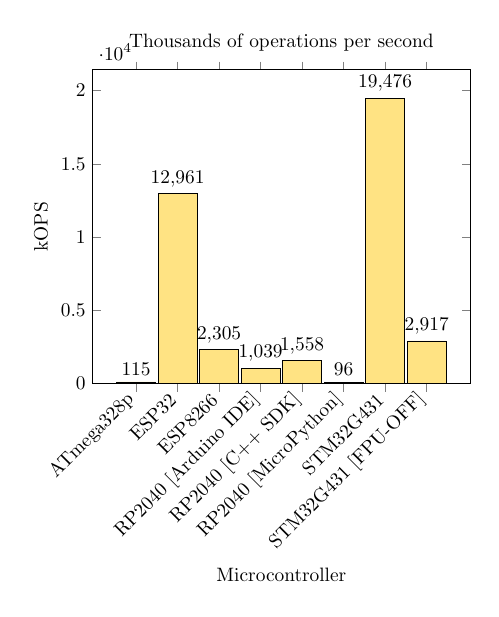
\begin{tikzpicture}[scale=0.7]
		\begin{axis}[
			x tick label style={rotate=45, anchor=east, align=right},
			title=Thousands of operations per second,
			xlabel={Microcontroller},
			ylabel={kOPS},
			ymin=0,
			ybar=5pt, % Adjust the space between bars
			enlarge x limits=0.15, % Add some breathing room between the bars
			bar width=20pt, % Adjust the width of the bars
			symbolic x coords={ATmega328p,ESP32,ESP8266,RP2040 [Arduino IDE],RP2040 [C++ SDK],RP2040 [MicroPython],STM32G431,STM32G431 [FPU-OFF]},
			xtick=data,
			nodes near coords,
			nodes near coords align={vertical},
			]
			\addplot[fill=Salomie10] coordinates  {
					(ATmega328p,115)
					(ESP32,12961)
					(ESP8266,2305)
					(RP2040 [Arduino IDE],1039)
					(RP2040 [C++ SDK],1558)
					(RP2040 [MicroPython],96)
					(STM32G431,19476)
					(STM32G431 [FPU-OFF],2917)
				};
		\end{axis}
	\end{tikzpicture}
	\caption{График максимальных значений тысяч операций в секунду у различных МК}\label{TestTimeP2}
\end{figure}



\begin{figure}[H]
	\centering
	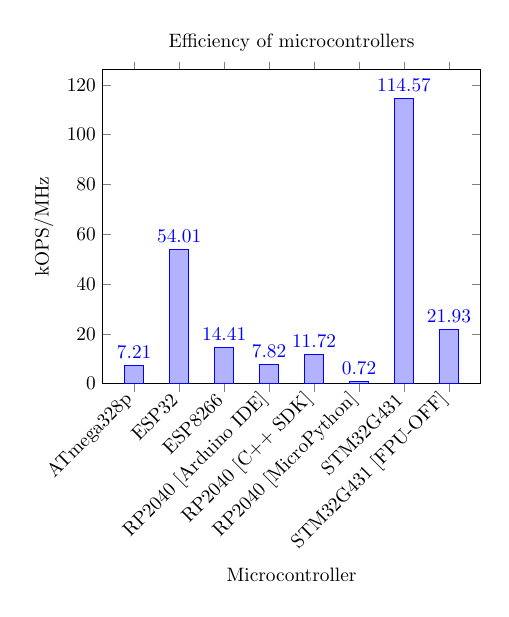
\begin{tikzpicture}[scale=0.7]
		\begin{axis}[
			x tick label style={rotate=45, anchor=east, align=right},
			title=Efficiency of microcontrollers,
			xlabel={Microcontroller},
			ylabel={kOPS/MHz },
			ymin=0,
			ybar, % Controls the space between bars
			symbolic x coords={ATmega328p,ESP32,ESP8266,RP2040 [Arduino IDE],RP2040 [C++ SDK],RP2040 [MicroPython],STM32G431,STM32G431 [FPU-OFF]},
			xtick=data,
			nodes near coords,
			nodes near coords align={vertical},
			]
			\addplot coordinates {(ATmega328p,7.205) (ESP32,54.007) (ESP8266,14.412) (RP2040 [Arduino IDE],7.815) (RP2040 [C++ SDK],11.717) (RP2040 [MicroPython],.723) (STM32G431,114.565) (STM32G431 [FPU-OFF],21.932)};
		\end{axis}
	\end{tikzpicture}
	\caption{ График значений тысяч операций в секунду на 1 мегагерц каждого МК}\label{TestTimeP3}
\end{figure}


В результате проведённых тестов было выяснено несколько интересных моментов связанных с микроконтроллерами. Как можно увидеть на рисунке 3.4 один процессор RP2040 с разными наборами средств разработки выдают различные результаты. Фаворитами теста являются МК  ESP32 с процессором Dual Xtensa LX6 от китайской компании «Espressif Systems» и микроконтроллер STM32G431 от компании «STMicroelectronics» с процессором Cortex M4. Чип STM был наиболее производительнее чем ESP32, хотя тактовая частота у ESP32 почти в двое выше STM, но нет значительного прироста в математических операциях. Стоит учесть STM вышел в лидеры по времени, из-за наличия аппаратных блоков операций с плавающей запятой (FPU) в процессоре.


% \usepackage{tabularray}
\begin{table}[H]
	\centering
	\caption{Таблица основных характеристик микроконтроллера STM32G431}\label{MCUData}

	\begin{tblr}{
		width = \linewidth,
		colspec = {Q[345]Q[541]},
		hlines,
		vlines,
		}
		\textbf{Parameter} & \textbf{Specification} \\
		Core               & ARM
		Cortex-M4                                   \\
		Operating
		Frequency          & Up
		to 170 MHz                                  \\
		Flash
		Memory             & Up
		to 512 KB                                   \\
		RAM                & Up
		to 128 KB                                   \\
		Digital
		I/Os               & Up
		to 82                                       \\
		Timers             & Multiple,
		including general purpose and advanced      \\
		DAC                & Yes,
		up to 2 channels                            \\
		ADC                & Yes,
		up to 16-bit                                \\
		Interfaces         & I2C,
		SPI, UART, USB, and others                  \\
		Operating
		Voltage            & 2.0
		V to 3.6 V                                  \\
		Temperature
		Range              & -40°C
		to +85°C                                    \\
		CAN
		Bus                & Yes,
		CAN
		2.0 (A, B)                                  \\
		Operational
		Amplifier (Op-amp) & Yes
	\end{tblr}
\end{table}


А также сопроцессора аппаратного ускорения математических операций «CORDIC».В результате контроллером системы управления был выбран чип STM32G431, в таблице \ref{MCUData} представлены основные характеристики данного чипа \citep{stmcordic}.

\subsection{Силовые ключи}
Силовые транзисторные ключи формируют трехфазный инвертер, для управления электродвигателем.  В данном случае транзисторные ключи задействованы для усиления PWM сигналов, поступающих от МК. Тип транзистора - N-канальный MOSFET транзисторы с индуцированным каналом. Такие транзисторы имеют очень малое сопротивление канала (Rds(on)). Это означает меньшие потери мощности при управлении нагрузкой, нагревание элемента будет меньше, что при одинаковых значениях параметров позволяют выбрать модели с меньшими габаритами. Силовые ключи должны соответствовать следующим требованиям:
\begin{itemize}
	\item Рабочее выходное напряжение более 24В;
	\item Рабочий температурный диапазон -30 до +80;
	\item Тип транзистора – MOSFET;
	\item Тип канала – n;
	\item Маленький размер элемента;
	\item Тип установки – поверхностный монтаж.
\end{itemize}
\begin{figure}[H]
	\centering
	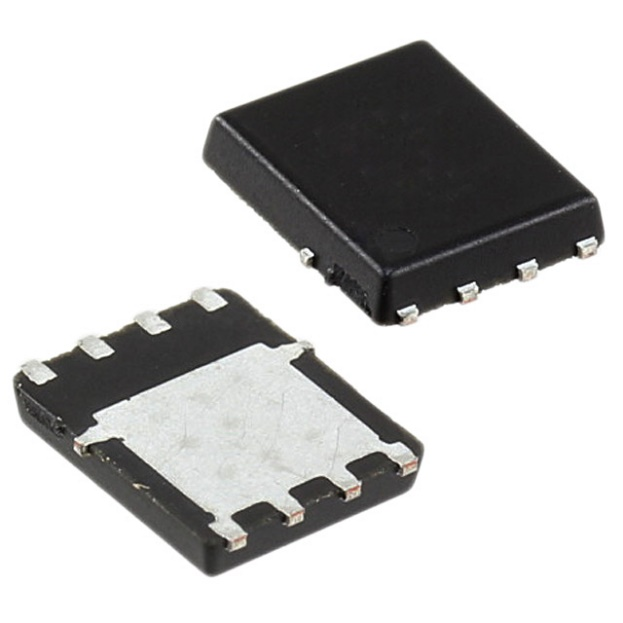
\includegraphics[width=0.5\textwidth]{Src/images/Transistir.png}
	\caption{Транзистор «SIR680DP»}
	\label{SIR680DP}
\end{figure}

Были выбраны транзисторы SIR680DP (Картинка \ref{SIR680DP}) от «Vishay Siliconix», SIR680DP - n- канальный MOSFET мощностью 80В / 100А. Они обладают высокой плотностью тока и низким сопротивлением открытого канала (RDS(on)), порядка 2.4 mΩ, остальные парметры находятся в таблице \ref{SIR680DPT}, что стало идеальной характеристикой подходящего элемента для применения с использованием ширинно-импульсной модуляции (PWM). Также важно отметить, что выбор компонентов был продиктован маленьким размером корпуса «PowerPAK-SO-8»,



% \usepackage{color}
% \usepackage{tabularray}
\begin{table}[H]
	\centering
	\caption{Таблица основных характеристик транзистор SIR680DP}\label{SIR680DPT}

	\begin{tblr}{
		width = \linewidth,
		colspec = {Q[547]Q[374]},
		hlines,
		vlines,
		}
		\textbf{Parameter}  & \textbf{Specification} \\
		Type                & N-Channel              \\
		Drain-Source
		Voltage (VDS)       & 80
		V                                            \\
		Gate-Source
		Voltage (VGS)       & ±
		20 V                                         \\
		Continuous
		Drain Current (ID)  & 100
		A (at TC = 25 °C)                            \\
		Pulsed
		Drain Current (IDM) & 200
		A (for
		100 μs)                                      \\
		Power
		Dissipation (PD)    & 104
		W (at TC = 25 °C)                            \\
		Operating
		Temperature Range   & -55°C
		to +150°C                                    \\
		RDS(on)
		max. at VGS = 10 V  & 0.0024
		Ω                                            \\
		Configuration       & Single                 \\
		Package             & PowerPAK
		SO-8
	\end{tblr}
\end{table}

\subsection{Драйвер силовых ключей}

Для облегчения управления мостовой транзисторной схемой инвертора используются драйвера. Их задача - преобразование маломощного сигнала, снимаемого с цифрового выхода МК, в сигнал с повышенным уровнем напряжения и мощности.

В данной реализации исполнительной систем использовались драйвера общего назначения L6385ED (Рисунок \ref{L6385ED}) производимые фирмой «STMicroelectronics». Данная микросхема является полумостовым драйвером. Один драйвер может управлять 2 силовыми транзисторами верхнего и нижнего уровня. Технические параметры L6385ED представлены в таблице \ref{L6385EDP}.

\begin{figure}[H]
	\centering
	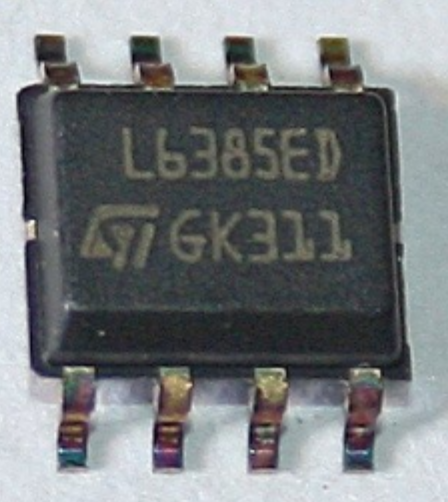
\includegraphics[width=0.3\textwidth]{Src/images/Driver.png}
	\caption{Драйвер L6385ED}
	\label{L6385ED}
\end{figure}

% \usepackage{color}
% \usepackage{tabularray}
\begin{table}[H]
	\centering
	\caption{Таблица основных характеристик драйвера L6385ED}\label{L6385EDP}

	\begin{tblr}{
		width = \linewidth,
		colspec = {Q[324]Q[317]},
		hlines,
		vlines,
		}
		\textbf{Parameter}            & \textbf{Specification} \\
		Maximum
		Operating Voltage             & 580V                   \\
		Supply
		Voltage                       & ±50V/nsec
		(across full temperature range)                        \\
		Driver
		Current Capability (Sourcing) & 400mA                  \\
		Switching
		Time (rise/fall)              & 50/30
		nsec                                                   \\
		Level
		of Input Control Signals      & CMOS/TTL
		Schmitt trigger with hysteresis and pull down          \\
		Under-voltage
		Lockout                       & On
		both lower and upper sections                          \\
		Bootstrap
		Diode                         & Internal
	\end{tblr}
\end{table}

\subsection{Передатчик шины данных}
Для обеспечения передачи данных между устройствами исполнительного управления, стратегического управления и других устройств целесообразно исользовать шину данных, для уменьшения количества соединительных проводников. Наиболее подходящим протоколом передачи данных является CAN шина, который является промышленным стандартом промышленной сети и не однократно использовалась для внедрения в роботы манипуляторы \citep{Megalingam2021}.
Главная причина использования шины CAN, это особенность в передачи данных, данные доступны всем устройствам, подключенным к сети. Возможна передача данных как одному, так и нескольким устройствам одновременно. На основе этого реализовывался вариант синхронизации всех исполнительных устройств, необходимых для своевременного начала движения \citep{stmfdcan}.
На основе выбранной модели микроконтроллера в главе 3.5 и технических данных из таблицы \ref{TCAN1462DRQ1T}, была выявлена аппаратная поддержка микроконтроллером CAN шины второго поколения - CAN FD.

\begin{figure}[H]
	\centering
	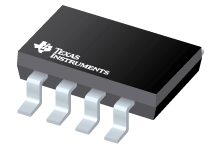
\includegraphics[width=0.3\textwidth]{Src/images/Trans.png}
	\caption{Передатчик TCAN1462DRQ1}
	\label{TCAN1462DRQ1}
\end{figure}

CAN-FD – это следующий этап развития классической шины CAN, которая обеспечивает более высокую скорость передачи данных и больший объем передаваемых данных в одном кадре, такое возможно из-за особенности передачи данных поля (CAN data) на скорости кратно превышающую скорость передачи заголовка, что может иметь значение вплоть до 8 Мбит/с.

Чтобы не ограничивать в возможной скорости передачу данных по шине CAN, был выбран передатчик TCAN1462DRQ1 (изображен на рисунке \ref{TCAN1462DRQ1}), передатчик выполняет усиление сигналов, защиту линии в случае повреждения CAN-шины, и регулировку скорости их передачи.

% \usepackage{color}
% \usepackage{tabularray}
\begin{table}[H]
	\centering
	\caption{Таблица основных характеристик передатчика TCAN1462DRQ1}\label{TCAN1462DRQ1T}

	\begin{tblr}{
		width = \linewidth,
		colspec = {Q[324]Q[317]},
		hlines,
		vlines,
		}
		\textbf{Parameter} & \textbf{Specification} \\
		Package            & SON-8
		(3x3mm)                                     \\
		Operating
		Temperature Range  & -40°C
		to +125°C                                   \\
		Supply
		Voltage Range      & 4.5V
		to 5.5V                                     \\
		Standby
		Current            & Typically
		5μA                                         \\
		Data
		Rate               & Up
		to 5 Mbps                                   \\
		ISO
		11898-2 Compliance & Yes
	\end{tblr}
\end{table}

\subsection{Преобразователь питания}
Из-за высокого потребления мини-компьютера, потребления достигает до 2.5А. По рекомендации производителя необходимо использовать отдельный DC – DC преобразователь. Источник питания должен соответствовать следующим требованиям:
\begin{itemize}
	\item Входное напряжение 24В;
	\item Преобразование DC-DC;
	\item Выходное напряжение 5В;
	\item Высокий выходной ток 3А и более.
\end{itemize}
\begin{figure}[H]
	\centering
	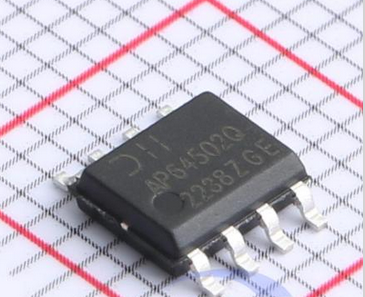
\includegraphics[width=0.3\textwidth]{Src/images/dc-dc.png}
	\caption{DC – DC микросхема АP64502QSP}
	\label{АP64502QSP}
\end{figure}
Была выбрана микросхема DC-DC Step-down преобразователя АP64502QSP, показанная на рис. \ref{АP64502QSP}. Преимущество импульсного преобразователя в высокой эффективности, не требующей теплоотвода, позволяет создавать компактные решения преобразования напряжения и тока.
Основным преимуществом выбора являляется способность преобразования большого тока 5A (таблица \ref{АP64502QSPT}), без использования внешних ключей и меньшего количество необходимых для работы данной микросхемы элементов \citep{AP64502Q}.



% \usepackage{color}
% \usepackage{tabularray}
\begin{table}[H]
	\centering
	\caption{Таблица основных характеристик DC-DC преобразователя АP64502QSP}\label{АP64502QSPT}

	\begin{tblr}{
		width = \linewidth,
		colspec = {Q[362]Q[499]},
		hlines,
		vlines,
		}
		\textbf{Parameter}    & \textbf{Specification} \\
		Input
		Voltage Range (VIN)   & 3.8V
		to 40V                                         \\
		Continuous
		Output Current        & 5A                     \\
		Programmable
		Switching Frequency   & 100kHz
		to 2.2MHz                                      \\
		Efficiency
		at Light Load         & Up
		to 85\%                                        \\
		Gate
		Driver Design         & Proprietary,
		for EMI Reduction                              \\
		Frequency
		Spread Spectrum (FSS) & Yes,
		for EMI Reduction                              \\
		Low-Dropout
		(LDO) Mode            & Yes                    \\
		Precision
		Enable Threshold      & For
		UVLO Adjustment                                \\
		Protection
		Features              & UVLO,
		OVP, Peak Current Limit, Thermal Shutdown
	\end{tblr}
\end{table}


\subsection{Функциональная схема системы управления мини роботом}

Функциональная схема системы управления мини роботом манипулятором показана на рис. \ref{FRobot}.
Главным управляющим элементом системы тактического управления, является управляющий МК STM32G431. К данному микроконтроллеру подключены все необходимые элементы.

Подключение Raspberry Pi Zero W2 (в роли стратегического устройства) к главному управляющему элементу STM32G431 возможно через два интерфейса UART, передача информация в текстовом виде и через SPI, для передачи сериализованных данных больших объёмов на большой скорости. Устройство Raspberry Pi задействует 5 линий ввода/вывода:

\begin{itemize}
	\item PA7 (SPI1\_MOSI) \rightarrow GPIO 12 (RPI\_MOSI);
	\item PA6 (SPI1 \_MISO) \rightarrow GPIO 13 (RPI\_MISO);
	\item PA5 (SPI1 \_SCLK) \rightarrow GPIO 14 (RPI\_SCLK);
	\item PA3 (UART2\_RX) \rightarrow RPI (RPI\_TX);
	\item PA2 (UART2\_TX) \rightarrow RPI (RPI\_RX).
\end{itemize}

Осуществление общения между устройствами исполнительной системы, используется передатчик шины CAN (TCAN1462) и передатчик задействует 2 линии ввода/вывода порта B, микроконтроллера STN32G431:
\begin{itemize}
	\item PB9 (FDCAN\_TX) \rightarrow CAN Transceiver (CAN\_TX);
	\item PB8 (FDCAN\_RX) \rightarrow CAN Transceiver (CAN\_RX);
\end{itemize}

Для обеспечения внешней связи используется передатчик интерфейса RS485 который подключается к 2 линии ввода/вывода порта A.
\begin{itemize}
	\item PA10 (UART2\_TX) \rightarrow RS485 (UART\_TX);
	\item PA9 (UART2\_RX) \rightarrow RS485 (UART\_RX);
\end{itemize}

Индикация состояния робота происходит через панель индикации и состоит из трёх светодиодов разного цвета и занимает 3 линии ввода/вывода порта B.
\begin{itemize}
	\item PB0 \leftarrow Indication Panel (LED\_YEL);
	\item PB1 \leftarrow Indication Panel (LED\_RED);
	\item PB2 \leftarrow Indication Panel (LED\_GRN);
\end{itemize}

Остальные свободные линии ввода/вывода портов B, отведены на блоки цифровых входов и выходов:
\begin{itemize}
	\item \textbf{Цифровые входы:}
	      \begin{itemize}
		      \item[$\circ$] PB11 \leftarrow DI (IN\_1);
		      \item[$\circ$] PB12 \leftarrow DI (IN\_2);
		      \item[$\circ$] PB13 \leftarrow DI (IN\_3);
		      \item[$\circ$] PB14 \leftarrow DI (IN\_4);
		      \item[$\circ$] PB15 \leftarrow DI (IN\_5);
		      \item[$\circ$] PA8 \leftarrow DI (IN\_6);
	      \end{itemize}
	\item \textbf{Цифровые выходы STN32G431:}
	      \begin{itemize}
		      \item[$\circ$] PB7 \rightarrow DO (OUT\_1);
		      \item[$\circ$] PB6 \rightarrow DO (OUT\_2);
		      \item[$\circ$] PB5 \rightarrow DO (OUT\_3);
		      \item[$\circ$] PB4 \rightarrow DO (OUT\_4);
		      \item[$\circ$] PB3 \rightarrow DO (OUT\_5);
		      \item[$\circ$] PA15 \rightarrow DO (OUT\_6);
	      \end{itemize}
\end{itemize}

Подключение всех частей системы производится на электронной плате с помощью пайки элементов. Также будут применены следующие разъёмы:
\begin{itemize}
	\item разъёмы для рабочего напряжения – XT30;
	\item Разъёмы для шины CAN - JST 1.25 PH 2;
	\item Штыревые разъёмы для остальной периферии - PBS.
\end{itemize}

Разъёмы XT30 обеспечивают надежное соединение и выдерживают значительные электрические нагрузки без потерь и риска возгорания из-за плохого контакта или перегрева.

Разъемы JST обеспечивают простоту подключения и отключения, что удобно при обслуживании и модернизации системы. Они предотвращают случайное обратное подключение, что может быть критично для предотвращения повреждений компонентов при монтаже.

Штыревые разъемы PBS подходят для подключения компонентов не требующих высоких токов, и при этом могут многократно использованы. Штыревые разъемы обеспечивают хороший контакт и простоту монтажа на печатной плате, что важно для быстрого прототипирования и наладки системы.


\begin{figure}[H]
	\begin{adjustbox}{addcode={\begin{minipage}{\width}}{\caption{
							Функциональная схема системы управления мини роботом
						}\label{FRobot}\end{minipage}},rotate=90,center}
		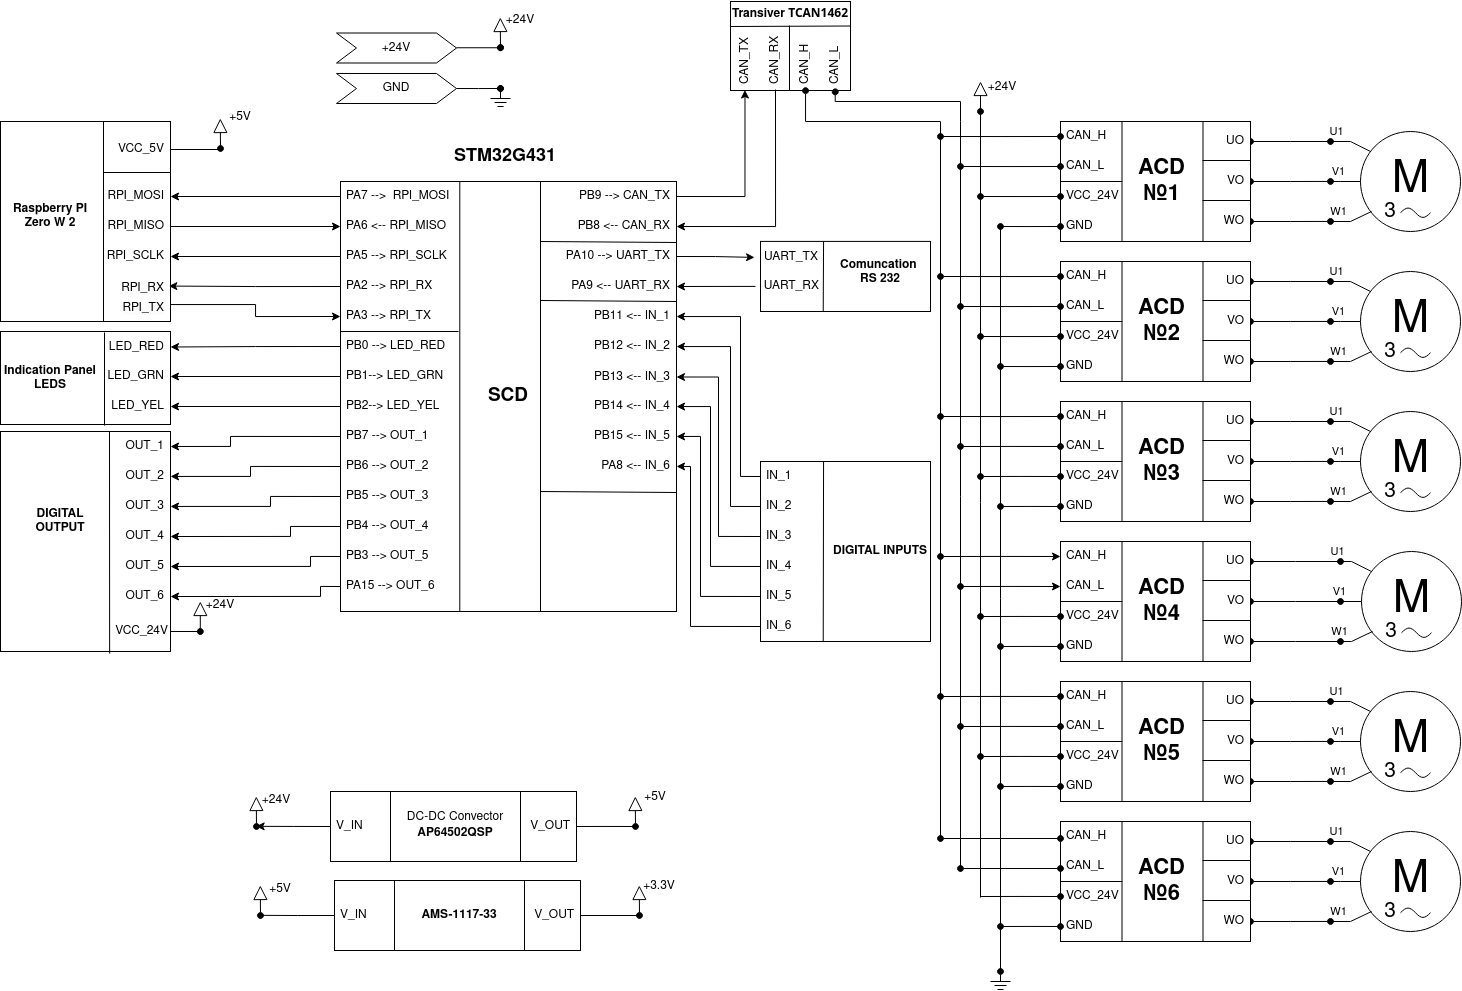
\includegraphics[width=0.85\paperheight]{Src/images/Func.drawio(1).png}
	\end{adjustbox}
\end{figure}

\subsection{Разработка функциональной схема системы исполнительного устройства}
Функциональна схема показана на рисунке \ref{FACD}/

Главным управляющим элементом обработки команд и генерации сигналов, системы исполнительной управления, является МК STM32G431. Генерация сигналов PWM происходит таймером и выводятся 6 канами сравнения, которые выведены на линии порта А, С и B:

\begin{itemize}
	\item PB15 \rightarrow HIN1;
	\item PB10 \rightarrow LIN1;
	\item PA12 \rightarrow HIN2;
	\item PB9 \rightarrow LIN2;
	\item PC13 \rightarrow HIN3;
	\item PA8 \rightarrow LIN3;
\end{itemize}
Драйвера усиливают сигнал от МК и подают на силовые ключевые транзисторы:
\begin{itemize}
	\item HIN1 \rightarrow HGV1;
	\item LIN1 \rightarrow LGV1;
	\item HIN2 \rightarrow HGV2;
	\item LIN2 \rightarrow LGV2;
	\item HIN3 \rightarrow HGV3;
	\item LIN3 \rightarrow LGV3;
\end{itemize}



Для измерения момента приложенного на двигатель, происходит измерения милы тока на каждой обмотке двигателя, измеряется падение напряжения путем подачи сигналов на входы операционных усилителей, которые встроенные в микроконтроллер 6 входов подключение производится:

\begin{itemize}
	\item PA1 \leftarrow +VSHUNT\_1;
	\item PA3 \leftarrow -VSHUNT\_1;
	\item PA7 \leftarrow -VSHUNT\_2;
	\item PA5 \leftarrow +VSHUNT\_2;  % Corrected from '-VSHUNT_2' to '+VSHUNT_2' for consistency
	\item PB0 \leftarrow -VSHUNT\_3;
	\item PB2 \leftarrow +VSHUNT\_3;  % Corrected from '-VSHUNT_3' to '+VSHUNT_3' for consistency
\end{itemize}

\begin{figure}[H]
	\begin{adjustbox}{addcode={\begin{minipage}{\width}}{\caption{
							Функциональная схема системы исполнительного управления
						} \label{FACD}
					\end{minipage}},rotate=90,center}
		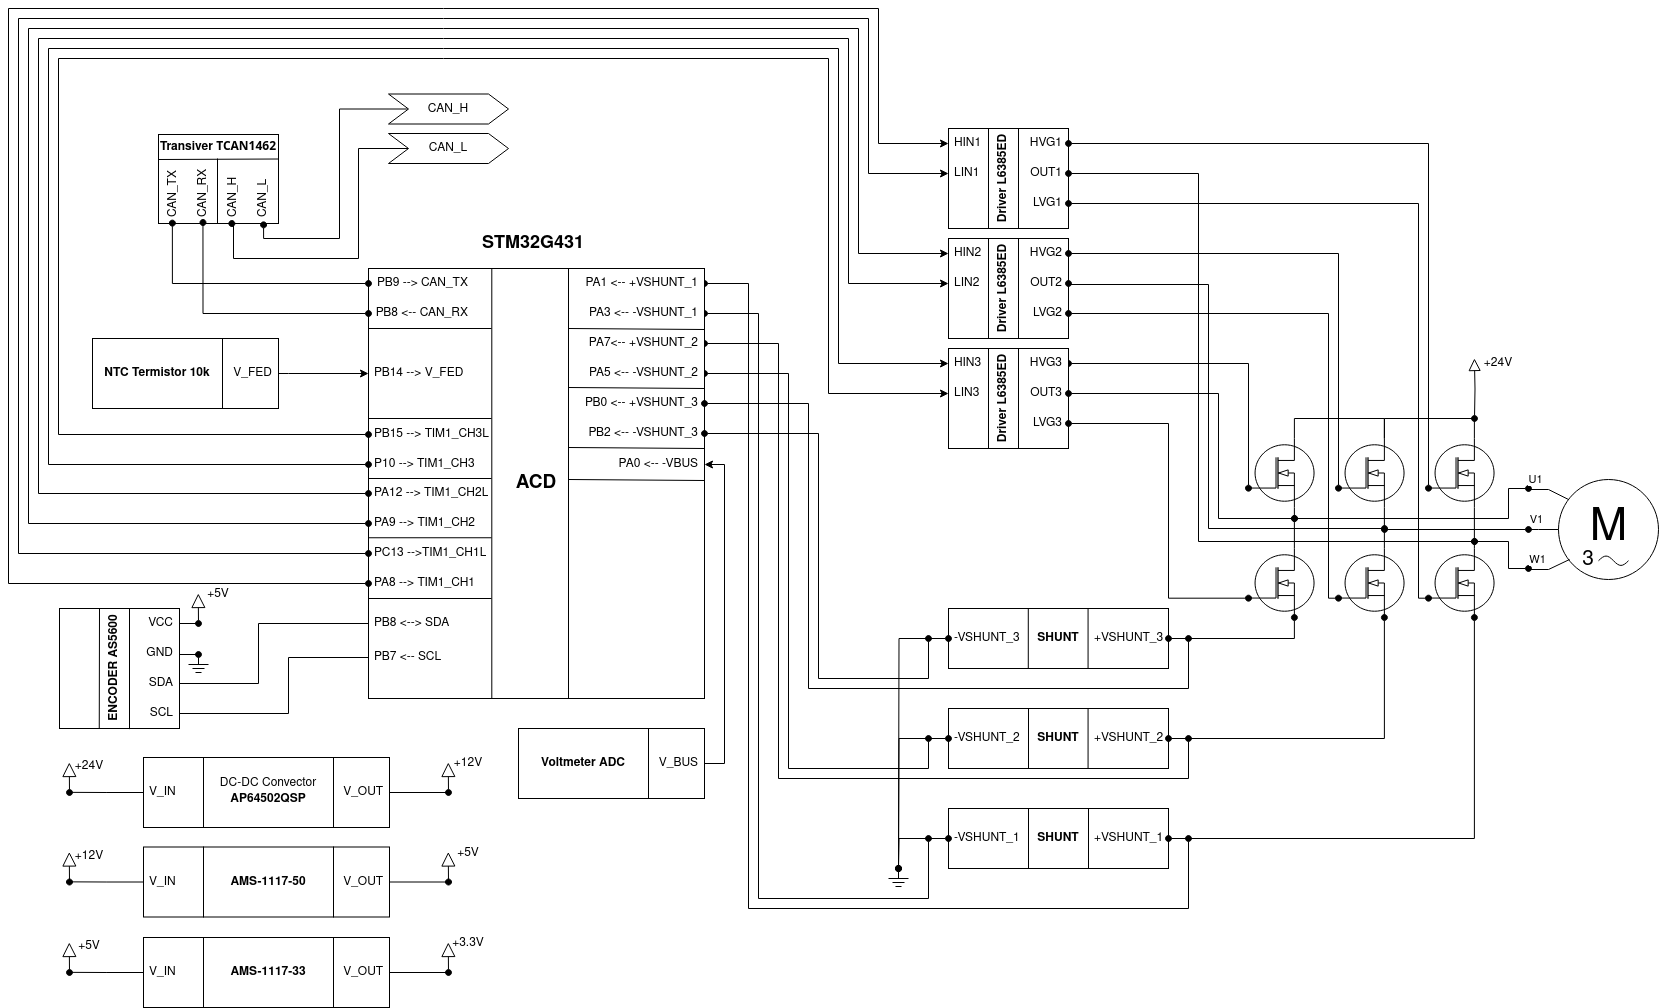
\includegraphics[width=0.85\paperheight]{Src/images/ACD (4).drawio.png}
	\end{adjustbox}
\end{figure}

Во избежание поломки устройства, предусмотрены две линии порта входа для подключения к АЦП микроконтроллера, один необходим для измерения температуры, датчик будет находится рядом с силовыми транзисторами, таким образом в случае перегрева, микроконтроллер предпринимает действия по установке в состояние ошибки. Второй АЦП используется для измерения поступающего рабочего напряжения, в случае выхода из диапазона рабочего напряжения, МК переходит в режим ошибки. АЦП расположены на линиях порта A и подключаются:

\begin{itemize}
	\item PA5 \rightarrow V\_FED;
	\item PA0 \rightarrow V\_BUS;
\end{itemize}


